\chapter{Interlude: Triangles in Triangles}
\label{cha:TrianglesInTriangles}
There are $\binom{n+2}{4}$ equilateral triangles with vertices in a triangular
region of the triangular grid with $n$ vertices on each side.
\begin{proof}
The following is a bijection without words from a choice of four integers
satisfying $1 \leq A < B < C < D \leq n + 2$
to equilateral triangles in the $n$-vertices-per-side triangular grid.

\noindent
\begin{center}
  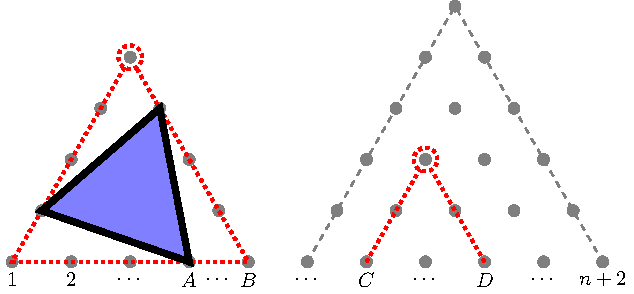
\includegraphics[scale=0.7]{figures/TrianglesInTriangles/assets/triangles_in_triangles_subset}
  \rule{\textwidth}{0.4pt}
  \vspace{0.5em}

  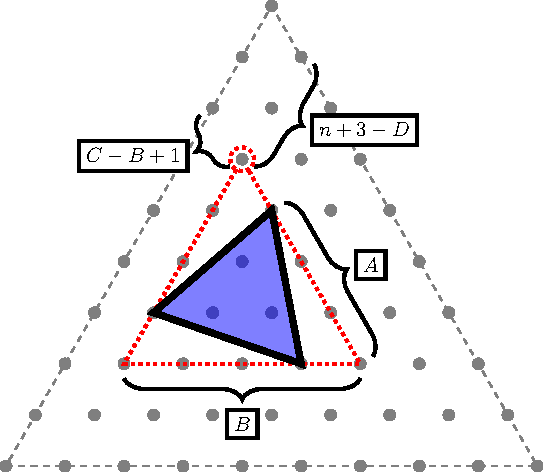
\includegraphics[scale=0.7]{figures/TrianglesInTriangles/assets/triangles_in_triangles}
\end{center}
\end{proof}
\begin{note}[Formerly the Abstract]
  We provide a visual proof of a bijection from $4$-element subsets of
  $\{1, 2, \dots, n + 2\}$ to triangles in the triangular grid where
  the orientation of the triangle is given by the smallest element of the subset,
  the size of its bounding triangle is by the second smallest element,
  and the position of its bounding triangle is given by the two largest elements.
  In this example, $n=10$, $A = 4$, $B = 5$, $C=6$, and $D=10$.
\end{note}
